\documentclass[10pt, letterpaper]{article}

% --- Packages ---
\usepackage{amsmath, amssymb, amsfonts} % Math symbols and environments
\usepackage[margin=1in]{geometry}     % Page margins
\usepackage{graphicx}                 % Include graphics
\usepackage[round]{natbib}            % Author-year citations
\usepackage{fancyhdr}                 % Custom headers/footers
\usepackage{url}                      % URL formatting
\usepackage{booktabs}                 % Better table rules
\usepackage{caption}                  % Figure/table captions
\usepackage{subcaption}               % Subfigures
\usepackage[utf8]{inputenc}           % Input encoding
\usepackage[T1]{fontenc}            % Font encoding
\usepackage{hyperref}                 % Clickable links/references
\hypersetup{
    colorlinks=true,
    linkcolor=blue,
    filecolor=magenta,      
    urlcolor=cyan,
    citecolor=blue,
    pdftitle={Bayesian Semiparametric Dynamic Frailty Models for Multiple Event Time Data},
    pdfauthor={Michael L. Pennell and David B. Dunson},
}

% --- Header/Footer Setup ---
\pagestyle{fancy}
\fancyhf{} % Clear default headers/footers
\fancyhead[L]{\small Pennell and Dunson: Bayesian Semiparametric Dynamic Frailty Models} % Adjust as needed
\fancyhead[R]{\small \thepage}
\renewcommand{\headrulewidth}{0pt} % No header rule
% Specific header for first page might need manual adjustment or \thispagestyle{fancy}

\newcommand{\correctToHere}{{\color{red}\large MATCHES ORIGINAL TEXT UP TO THIS POINT. CONTINUE CHECKING FROM HERE.}}
\graphicspath{{graphics/}}

% --- Title and Author Info ---
\title{REPRODUCTION OF LATEX ATTEMPT WITH GEMINI 2.5: Bayesian Semiparametric Dynamic Frailty Models for Multiple Event Time Data}

\author{
    Michael L. Pennell$^{1,2,*}$ \and David B. Dunson$^2$ \\\\ % Use \\ for line breaks
    $^1$Department of Biostatistics, University of North Carolina at Chapel Hill,\\
    Chapel Hill, North Carolina 27599, U.S.A. \\\\
    $^2$Biostatistics Branch, MD A3-03, National Institute of Environmental Health Sciences,\\
    P.O. Box 12233, Research Triangle Park, North Carolina 27709, U.S.A. \\\\
    $^*$email: \href{mailto:pennell@niehs.nih.gov}{pennell@niehs.nih.gov}
}

\date{December 2006} % Or \date{} to omit date

% --- Document Start ---
\begin{document}

% --- First Page Special Headers ---
% This attempts to mimic the journal header on page 1 (1044)
\fancypagestyle{plain}{% Redefine plain style used by \maketitle
  \fancyhf{}%
  \fancyhead[L]{BIOMETRICS 62, 1044--1052 \\ December 2006}%
  \fancyhead[R]{DOI: 10.1111/j.1541-0420.2006.00571.x}%
  \renewcommand{\headrulewidth}{0pt}%
}
\maketitle
\thispagestyle{plain} % Apply the redefined plain style to the first page

% --- Abstract ---
\begin{abstract}
\noindent \textbf{SUMMARY.} Many biomedical studies collect data on times of occurrence for a health event that can occur repeatedly, such as infection, hospitalization, recurrence of disease, or tumor onset. To analyze such data, it is necessary to account for within-subject dependency in the multiple event times. Motivated by data from studies of palpable tumors, this article proposes a dynamic frailty model and Bayesian semiparametric approach to inference. The widely used shared frailty proportional hazards model is generalized to allow subject-specific frailties to change dynamically with age while also accommodating nonproportional hazards. Parametric assumptions on the frailty distribution are avoided by using Dirichlet process priors for a shared frailty and for multiplicative innovations on this frailty. By centering the semiparametric model on a conditionally conjugate dynamic gamma model, we facilitate posterior computation and lack-of-fit assessments of the parametric model. Our proposed method is demonstrated using data from a cancer chemoprevention study.
\end{abstract}

% --- Keywords ---
\noindent \textbf{KEY WORDS:} Breast cancer; Chemoprevention; Dirichlet process; Nonparametric Bayes; Palpable tumors; Survival analysis; Tumor multiplicity data.

\section{AI Tools Used}

\href{https://aistudio.google.com/app/prompts?state=%7B%22ids%22:%5B%221yQGdmKIe0PcuxkvLv0s_LrTA6HtqqG3j%22%5D,%22action%22:%22open%22,%22userId%22:%22106051103597265536066%22,%22resourceKeys%22:%7B%7D%7D&usp=sharing}{Gemini session}

\section{Introduction}

Many biomedical studies are designed to assess covariate effects on the time to recurrence of health-related outcomes, such as infections, hospitalizations, or recurrences of disease. For example, data of this type are collected in chemoprevention and carcinogenicity studies measuring the rate of appearance of palpable tumors of the skin and breast of mice \citep{Gail1980, Forbes1998, Dunson2000}. In these experiments, a rich set of data is available for each mouse, including times of appearance of each lesion, total number of tumors, and time of death.

A number of methods have been proposed to analyze tumor multiplicity data including recent work by \citet{Dunson2000b} and \citet{Sinha2002b}. These articles relied on frailty-type models \citep{Vaupel1979, Clayton1985} to accommodate baseline heterogeneity in risk of developing tumors. In these models, random effects (or frailties) measure an animal's risk relative to that of other individuals in the population, accounting for covariates. Standard shared and multivariate \citep{Sargent1998} frailty models treat the frailties as time-independent factors, and hence do not allow a subject's risk to evolve dynamically as they age. Such formulations may be overly restrictive when applied to tumorigenicity data, because biological changes occurring with age result in complex and unanticipated trends in susceptibility to tumor development. A likely trend is that animals getting tumors relatively early may not be at higher risk later in life.

Recently, several authors have proposed more flexible, dynamic formulations. \citet{Yue1997} and \citet{Yau1998} introduced a proportional hazard model for interrecurrence times in which a subject's frailty changes following each event, and \citet{Lam2002} developed a related approach for the proportional odds model. In tumorigenicity studies, a time-varying frailty structure may be more realistic because it is more natural to model individual-specific risk as changing with age instead of according to previous occurrences of tumors. Relevant methods have been proposed by \citet{Henderson2003}, who developed a longitudinal Poisson regression model with gamma frailties that vary with time, and \citet{Paik1994}, who proposed a proportional hazards frailty model with a time-specific random factor. Although promising, these methods involve complicated likelihoods and difficult computation, particularly when one considers generalizations (e.g., for joint modeling).

Bayesian approaches have several advantages, including ease of computation via MCMC, ability to incorporate prior information (e.g., from historical controls), and exact inferences on different aspects of the tumor response (time to first tumor, total tumor burden, etc). In the Bayesian literature, there has been limited consideration of dynamic frailty models and methods for multiple event time data in general. For recent Bayesian references on frailty models for multiple event time and multivariate survival data, refer to papers by \citet{Gustafson1997}, \citet{Sahu1997}, \citet{Walker1997}, \citet{Sargent1998}, \citet{Aslanidou1998}, \citet{Sinha1998}, \citet{Chen2002}, \citet{Dunson2004}, \citet{Sinha2004}, as well as a review by \citet{Ibrahim2001}. \citet{Harkanen2003} proposed an innovative approach based on a model that allows subject-specific frailty trajectories to vary according to a latent class structure. In many settings, including animal tumorigenicity studies, it may be more natural to suppose that the age-specific risk trajectories vary according to a continuum, with each subject potentially having their own unique pattern.

Motivated by the tumor multiplicity application, we propose a Bayesian semiparametric dynamic frailty model. Our methodology generalizes the shared frailty model to allow time-varying frailties and regression coefficients. In addition, we use a multiplicative parameterization to introduce autocorrelation and smooth the time trajectories. To improve flexibility, we consider a nonparametric treatment of the frailty distribution using a model which is related to the Dirichlet process (DP) mixture \citep{Antoniak1974}. For references on related approaches using DP mixtures in Bayesian analyses, refer to \citet{West1994}, \citet{Bush1996}, \citet{Mukhopadhyay1997}, \citet{Muller1997}, \citet{Kleinman1998}, and \citet{Dominici2001}. In addition, an alternative nonparametric approach for recurrent event time data was proposed by \citet{Ishwaran2004}. In this article, we use DP priors to allow uncertainty in the distributions of a shared frailty and multiplicative innovations on this frailty. By centering the semiparametric model on a conditionally conjugate dynamic gamma model, we facilitate posterior computation and lack-of-fit assessments of the parametric model using predictive distributions.

Section 2 proposes the model and prior structure. Section 3 outlines an MCMC algorithm for posterior computation. Section 4 applies the method to data from a cancer chemoprevention study, and Section 5 discusses the results.

\section{Dynamic Frailty Model}

\subsection{Model Specification and Frailty Structure}

\correctToHere

Consider a study measuring the times of occurrence of repeated events within $n$ subjects. The rate of event occurrence for subject $i$ ($i = 1, \dots, n$) at time $t$ is denoted $\Lambda_i(t)$. We partition the time axis into $M$ finely spaced intervals, $T_1, T_2, \dots, T_M$, where $T_j = (\tau_{j-1}, \tau_j]$, $0 = \tau_0 < \tau_1 < \tau_2 < \dots < \tau_M$, and $\tau_M$ is the maximum follow-up time in the study. The intervals are chosen to be sufficiently narrow so that it can be assumed that $\Lambda_i(t) = \lambda_{ij}$ for all $t \in T_j$, $j = 1, \dots, M$.
Suppose that subject $i$ is followed for $t_i$ time units, where $t_i \in T_{M_i}$ and $M_i \le M$. Under these specifications, let $\xi_i = (\xi_{i1}, \dots, \xi_{iM_i})'$ denote a vector of time-varying frailties for subject $i$, and let $x_{ij} = (x_{ij1}, \dots, x_{ijp})'$ be a vector of $p$ predictors for subject $i$ and time interval $T_j$. We focus on models having the following structure:
\begin{equation} \label{eq:1}
\lambda_{ij} = \xi_{ij} \lambda_{0j} g(x_{ij}' \beta_j),
\end{equation}
where $\lambda_{0j}$ is the baseline hazard for the $j$th interval, $g(\cdot)$ is a known link function mapping from $\mathbb{R}^p \to \mathbb{R}^+$, and $\beta_j$ are interval-specific regression parameters. We further express the baseline hazard as $\lambda_{0j} = \lambda_{0j}^* \Delta_j$, where $\lambda_{0j}^*$ is an initial guess at the baseline hazard (e.g., estimated from historical control data or based on expert elicitation) and $\Delta_j$ is a multiplicative deviation from this guess.

Similar to what is done by \citet{Paik1994}, the frailties are decomposed into time-independent and time-dependent components:
\begin{equation} \label{eq:2}
\xi_{ij} = \phi_i \prod_{h=1}^{j} \phi_{ih},
\end{equation}
where $\phi_i$ is a subject-specific shared frailty and $\phi_{ih}$ is the multiplicative innovation over time interval $h$. This multiplicative structure provides a convenient framework for imposing autocorrelation among the frailties. To demonstrate this feature, consider a model in which $\phi_i \stackrel{iid}{\sim} G(\psi_1, \psi_1)$ independently of $\phi_{ih} \stackrel{iid}{\sim} G(\psi_2, \psi_2)$, $h = 1, \dots, M_i$. Given these distributions, the correlation between frailties from intervals $j$ and $j + d$ ($d > 0$) is
\begin{equation} \label{eq:3}
\text{corr}(\xi_{ij}, \xi_{i(j+d)}) = \frac{\psi_1^2 \{ (1 + \psi_1)(1 + \psi_2)^j - \psi_1 \psi_2^j \}}{\sqrt{\{ (1 + \psi_1)(1 + \psi_2)^j - \psi_1 \psi_2^j \} \{ (1 + \psi_1)(1 + \psi_2)^{j+d} - \psi_1 \psi_2^{j+d} \}}}
\end{equation}
Under the above model, $\psi_1$ provides an overall measure of between-subject heterogeneity while $\psi_2$ can be thought of as both a smoothing parameter for the frailty trajectories and a measure of temporal heterogeneity within each subject.

Although we have observed that this dynamic gamma model performs well with some data, it can lead to spurious inferences when the actual distributions of the frailty components are distinctly nongamma. For example, \citet{Walker1997} demonstrated that frailty distributions may differ across predictor level resulting in multimodal distributions when all the frailties are pooled together. With this in mind, we propose a semiparametric model that is flexible to unanticipated trends in the frailty.

For subject $i$ and interval $T_j$, let $r_{ij}$ denote the time at risk and let $N_{ij}$ denote the number of events experienced. Then, under expressions \eqref{eq:1} and \eqref{eq:2} with a DP specification for the distributions of $\phi_i$ and $\phi_{ih}$, we have:
\begin{equation} \label{eq:4}
\begin{aligned}
 N_{ij} &\stackrel{\text{ind.}}{\sim} \text{Poisson}\left(\phi_i \left(\prod_{h=1}^{j} \phi_{ih}\right) \Delta_j \lambda_{0j}^* g(x_{ij}' \beta_j) r_{ij}\right) \\
 \phi_i &\stackrel{\text{ind.}}{\sim} G_1 \\
 \phi_{ih} &\stackrel{\text{ind.}}{\sim} G_{h+1} \\ 
 G_1 &\sim \mathcal{D}(\alpha_{01} G_{01}) \\
 G_{j+1} &\sim \mathcal{D}(\alpha_{02} G_{02}), 
\end{aligned}
\end{equation}
where $\mathcal{D}(\alpha G_0)$ denotes the DP centered on $G_0$ with precision $\alpha$, and we assume $G_{01}$ is $G(\psi_1, \psi_1)$ and $G_{02}$ is $G(\psi_2, \psi_2)$. This structure is centered on the dynamic gamma frailty model described above, but we allow the true frailty distribution to deviate from the parametric form. The amount of uncertainty in the gamma assumption for the two frailty components is controlled by the hyperparameters $\alpha_{01}$ and $\alpha_{02}$, with small values of these parameters corresponding to little faith in the gamma forms.

Because $G_1, G_2, \dots, G_{M+1}$ are modeled as discrete distributions under the DP \citep{Blackwell1973}, there will be common values of the shared frailties and multiplicative innovations across subjects under \eqref{eq:4}. Thus, our method identifies clusters of subjects whose genetic traits convey a similar level of susceptibility at the outset of the study as well as clusters of subjects who experience similar increases in their susceptibility over each time interval. These latter clusters may identify subjects who experienced similar, unobserved events, such as subjects who experienced changes in gene expression that increased their susceptibility to developing new tumors.

\subsection{Priors for Model Deviations and Regression Parameters}

As with the frailties, the multiplicative deviations from the initial baseline hazard estimates are separated into time-dependent and time-independent components:
\begin{equation} \label{eq:5}
\Delta_j = \nu_0 \prod_{h=1}^{j} \nu_h.
\end{equation}
Assuming $\nu_0 \sim G(\kappa, \kappa)$ and $\nu_h \stackrel{iid}{\sim} G(\psi_3, \psi_3)$ for $h = 1, \dots, M$, we have a convenient structure for introducing autocorrelation among the model deviations
\begin{equation} \label{eq:6}
\text{corr}(\Delta_j, \Delta_{j+d}) = \frac{\psi_3^d \{ (1 + \kappa)(1 + \psi_3)^j - \kappa \psi_3^j \}}{\sqrt{\{ (1 + \kappa)(1 + \psi_3)^j - \kappa \psi_3^j \} \{ (1 + \kappa)(1 + \psi_3)^{j+d} - \kappa \psi_3^{j+d} \}}},
\end{equation}
where $\kappa$ controls the degree of shrinkage of the posterior toward $\lambda_{0j}^*$, and $\psi_3$ measures smoothness in the deviations from the prior estimate. An appealing feature of this prior in the context of the tumor multiplicity application is that the prior variance increases with time. In many applications, events are known to be rare early and one can obtain a good prior estimate early on, but at later times there is much more uncertainty.

Although many other correlated prior processes have been proposed for the baseline hazard (cf. \citealp{Gamerman1991}; \citealp{Arjas1994}; \citealp{Gustafson2003}), our proposed structure is practically appealing for complex models because it retains the conditional conjugacy properties of the gamma process \citep{Kalbfleisch1978} without the need to introduce any additional latent variables (cf. \citealp{NietoBarajas2002}). These properties are highlighted in the following section on posterior computation.

A similar prior structure can be used to provide smooth trajectories for predictor effects. This technique is an alternative to dynamic covariate models based on random walks (cf. \citealp{Gamerman1991}; \citealp{Sargent1997}) and can simplify computation in certain applications. We consider the typical exponential link function, $g(x_{ij}'; \beta_j) = e^{x_{ij}' \beta_j}$. However, our priors are developed in terms of the following reparameterization of $\beta_j = (\beta_{j1}, \dots, \beta_{jp})'$:
\[
\gamma_{jk} = e^{\beta_{jk}} = \prod_{l=1}^{j} \gamma_{lk},
\]
where $\gamma_{jk} = \lambda_i(t; x_{ijk} = c+1) / \lambda_i(t; x_{ijk} = c)$ for $t \in T_j$ is the multiplicative change in hazard (i.e., hazard ratio) at time $t$ attributable to a unit increase in the $k$th predictor, and $\gamma_{lk} = \gamma_{jk} / \gamma_{(j-1)k}$ is the multiplicative innovation in this hazard ratio experienced over time interval $T_l$. In the absence of prior information about the effect of the $k$th predictor, it is reasonable to assume $\gamma_{lk} \stackrel{iid}{\sim} G(\psi_4, \psi_4)$ priors for the multiplicative increments on the hazard function. The prior is centered on no effect for a predictor with the degree of shrinkage and smoothness in the regression function controlled by the hyperparameter $\psi_4$, as is clear from the following expression:
\begin{equation} \label{eq:7}
\text{corr}(\gamma_{jk}, \gamma_{(j+d)k}) = \frac{\psi_4^d \{ (1 + \psi_4)^j - \psi_4^j \}}{\sqrt{\{ (1 + \psi_4)^j - \psi_4^j \} \{ (1 + \psi_4)^{j+d} - \psi_4^{j+d} \}}}
\end{equation}
In cases in which one has prior information about the regression function, the prior structure above could be used to model multiplicative deviations from these initial estimates. This approach is closely related to our priors for the baseline hazard. Another extension that may be useful in some applications would be to allow the level of smoothing to vary across predictors. These generalizations are straightforward and we focus on the simple case for ease of exposition.

\subsection{Elicitation of Hyperpriors}

To reduce the sensitivity of analyses to subjectively chosen hyperparameters, we consider the use of hyperpriors in building our dynamic frailty model. A priori we assume that $\psi_1 \sim G(a_1, b_1)$ and $\psi_2 \sim G(a_2, b_2)$ to obtain some information from the data about the variance components of the frailties. Although a diffuse prior would be reasonable for $\psi_1$, allowing the level of between-subject heterogeneity to be determined by the data, we recommend using an informative prior for $\psi_2$ centered on values which reflect the expected amount of correlation between Poisson counts from adjacent time intervals.

One could additionally specify gamma hyperpriors for $\psi_3$ and $\psi_4$, but preliminary results suggest that it can be difficult to specify a prior that ensures sufficient smoothing of the baseline hazard and predictor effects, because the likelihood tends to dominate the prior even for moderate sample sizes. Thus, to avoid overfitting, we recommend choosing values of $\psi_3$ and $\psi_4$ which reflect both one's a priori intuition about the level of autocorrelation between time intervals and one's confidence in the initial guess of the baseline hazard. We also recommend performing a sensitivity analysis of this choice. Hyperpriors for $\alpha_{01}$ and $\alpha_{02}$ may also be elicited to determine the amount of deviation from the gamma frailty structure in the data, though we prefer to fix these parameters to avoid overparameterization.

\section{Posterior Computation}

\subsection{MCMC Methodology}

In applications with moderate to large sample sizes and lengthy follow-ups, our model will result in a large number of latent variables and unknown parameters. Fortunately, due to the conditionally conjugate structure of the priors, computation can proceed fairly easily using a hybrid MCMC algorithm consisting of Gibbs and Metropolis-Hastings steps \citep{Gelfand1990, Tierney1994}. For the complete details regarding the full conditional posterior distributions and updating algorithm of our MCMC, please see the technical report associated with this article which is available at \url{http://www.tibs.org/biometrics}.

For simplicity, our methods assume that data are right censored and that censoring is noninformative. To modify our MCMC algorithm to accommodate interval-censored data, one can simply include data augmentation steps for sampling the exact event times for interval-censored observations. In addition, dependent censoring may be accommodated by incorporating the time-varying frailty as a predictor in a model for the censoring time. These models would generalize the shared frailty models of \citet{Liu2004}.

Our proposed MCMC methodology performed well when applied to simulated data. Posterior estimates of the time-varying hazard ratios and future predictions of the hazard function tended to agree closely with the true values, even when the prior for the baseline hazard was poorly specified. As expected, results were somewhat sensitive to the prior when sample sizes were small. However, robustness improved with increasing sample sizes, likely reflecting the borrowing of information across time and hyperprior structure.

\subsection{Identifiability and Computational Issues}

As for most latent variable models, some identifiability restrictions are needed. In practice, $\nu_1$ and $\phi_{i1}$ should be fixed at 1, because these parameters have the same contributions to likelihood as $\nu_0$ and $\phi_i$, $i=1, \dots, n$. We also recommend fixing $\nu_0$ because there may be a tendency for weak identifiability between $\nu_0$ and the mean of $G_1$, leading to slow mixing of the MCMC algorithm.

Another issue in implementation is the choice of knots for the piecewise constant hazard. The typical frequentist approach of choosing intervals at the unique failure times (e.g., \citealp{Breslow1974}) is inappropriate from a Bayesian perspective, because it involves using the data to choose priors. By choosing autocorrelated priors, which borrow information across intervals, our approach allows for tightly spaced intervals. However, we recommend choosing knots so that intervals are at least as wide as the interexam times; data are not informative about changes on a finer scale, and the computational burden increases with the number of intervals.

\section{Chemoprevention Application}

\subsection{Data Analysis}

We illustrate our approach using data from a study of the effect of canthaxanthin, a carotenoid found in fruits and vegetables, on chemically induced mammary carcinogenesis \citep{Grubbs1991}. This data set has previously been used as an example by both \citet{Kokoska1993} and \citet{Dunson2000b}. The study consisted of 119 Sprague-Dawley rats administered one of four diets beginning at 34 days of age: (1) 3390 mg/kg canthaxanthin, (2) 1130 mg/kg canthaxanthin, (3) 328 mg/kg retinyl acetate, or (4) vehicle control. There were 30 rats in treatment groups 1--3 and 29 in group 4. At age 55 days, each rat was administered 15 mg of a known carcinogen DMBA by gavage. Regular palpations began at 75 days of age and, in general, were performed twice a week until 235 days of age, or 180 days following administration of DMBA.

Our analysis focused on the tumor occurrence times, as measured from DMBA administration, of rats in treatment groups 1, 2, and 4. We partitioned the study period into 24 time intervals, with each interval having a length of 1 week except for the first and last intervals (22 and 4 days, respectively). When the animals died naturally or were sacrificed at the end of the study period, an extensive pathological examination was conducted to find tumors that may be undetectable by palpation. For this reason, we allowed for a multiplicative increase in the baseline hazard of tumor detection at the final examination by introducing an additional parameter, $\omega$, into our model. Thus, the model we used has the following form:
\begin{equation} \label{eq:8}
\lambda_{ij} = \xi_{ij} \nu_0 \lambda_{0j}^* \omega^{I_{ij}} \prod_{h=1}^{j} \nu_h \prod_{k=1}^{2} \gamma_{jk}^{x_{ik}}, 
\end{equation}
where $I_{ij} = 1$ if $j = M$ and 0 otherwise and $x_{ik} = 1$ if subject $i$ is in treatment group $k$ and 0 otherwise, $k = 1, 2$. Assigning a $G(a_\omega, b_\omega)$ prior to $\omega$ results in the conditional posterior,
\begin{equation} \label{eq:9}
\pi(\omega | \cdot) = G \left( a_\omega + \sum_{i=1}^{n} N_{iM}, b_\omega + \sum_{i=1}^{n} r_{iM} \phi_i \nu_0 \lambda_{0M}^* \prod_{h=1}^{M} \nu_h \prod_{k=1}^{2} \gamma_{Mk}^{x_{ik}} \right).
\end{equation}

In this study of cancer initiation, the retinyl acetate group (3) can be considered as a second control group, because it is known that this treatment is only effective in decreasing promotion \citep{Grubbs1991}. Thus, these data were used to choose the prior for the baseline hazard. In particular, we fit a Poisson regression model with a cubic polynomial in time to the group 3 data and used the resulting fitted curve as $\lambda_{0j}^*$. We chose $G(5, 0.5)$ and $G(25, 0.5)$ priors for $\psi_1$ and $\psi_2$, respectively, to express belief in low between- and within-subject heterogeneity but high levels of autocorrelation among the frailties. Because tumor incidence should be negligible in the first 3 weeks of the study, we assumed $\gamma_{11} = \gamma_{12} = 1$. In addition, to express modest confidence in the gamma frailty assumptions, we set $\alpha_{01} = \alpha_{02} = 5$. Finally, we let $\psi_3 = \psi_4 = 50$ to induce high levels of smoothing in both the baseline hazard and treatment effects, and set $a_\omega = 3$ and $b_\omega = 1$ to reflect our a priori belief that more tumors are observed in the exam following sacrifice.

Using our MCMC methodology, we ran a chain of 55,000 iterations with the first 5000 discarded as a burn-in. To reduce storage requirements, every 10th observation was saved to thin the chain. It took approximately 4 hours to complete a Matlab (version 7.0) program run in batch on the statistical server at UNC-Chapel Hill (20 1.05 GHz processors).

Figure \ref{fig:1} provides the mean and pointwise 95\% credible intervals for the hazard ratios comparing the canthaxanthin dose groups to control. Although the hazard ratios are initially near one, as time progresses they decrease toward a plateau between weeks 10--26. The posterior mean and 95\% credible interval for the average hazard ratio over this interval is $\bar{\gamma}_{[10,26]2} = 0.553$ (0.343, 0.863) in the low-dose group and $\bar{\gamma}_{[10,26]1} = 0.489$ (0.304, 0.758) in the high-dose group. In addition, the estimated posterior probabilities of a chemopreventive effect in the two groups for this interval are $\text{Pr}(\bar{\gamma}_{[10,26]2} < 1 | \mathbf{Y}) = 0.995$ and $\text{Pr}(\bar{\gamma}_{[10,26]1} < 1 | \mathbf{Y}) = 0.999$, with $\text{Pr}(\bar{\gamma}_{[10,26]2} > \bar{\gamma}_{[10,26]1} | \mathbf{Y}) = 0.676$, suggesting highly significant, but similar, effects overall in the two dose groups.

\begin{figure}[htbp]
    \centering
    \begin{subfigure}[b]{0.8\textwidth}
        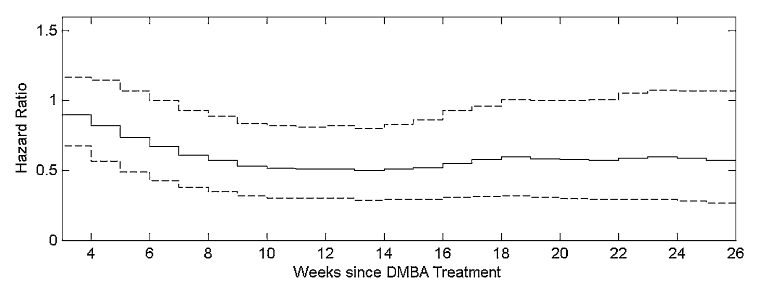
\includegraphics[width=\textwidth]{figure1a.png} % Placeholder
        \caption{}
        \label{fig:1a}
    \end{subfigure}
    \vfill
    \begin{subfigure}[b]{0.8\textwidth}
        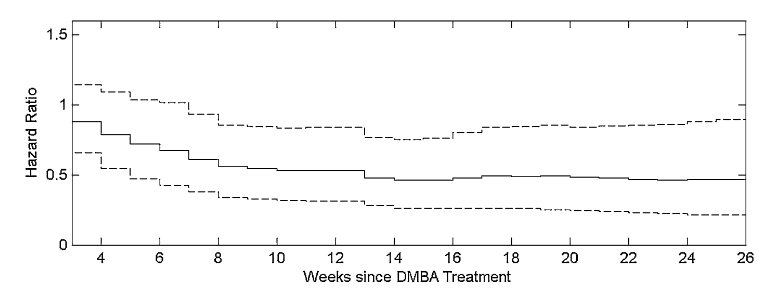
\includegraphics[width=\textwidth]{figure1b.png} % Placeholder
        \caption{}
        \label{fig:1b}
    \end{subfigure}
    \caption{Posterior means (---) and pointwise 95\% credible intervals (- - -) for hazard ratios comparing rats fed (a) 1130 mg/kg and (b) 3390 mg/kg canthaxanthin to rats administered a vehicle control diet.}
    \label{fig:1}
\end{figure}

As discussed by \citet{Kokoska1993} and \citet{Dunson2000b}, in the presence of a significant effect on tumor incidence, there is typically interest in assessing which aspects of the tumor response profile are most affected. In particular, tumor biologists wish to distinguish effects on multiplicity (total number of tumors) and latency (time to tumor onset). In our model, the effects of treatment group $k$ on multiplicity may be evaluated by computing the posterior probability $P_{Mk} = \text{Pr}(\Lambda_{kM} / \Lambda_{0M} < 1 | \mathbf{Y})$, where $\Lambda_{kM}$ is the cumulative hazard at sacrifice for an animal in treatment group $k$ ($k=1, 2$) with frailty $\xi_i = 1$ (i.e., the prior mean in the dynamic gamma model) and $\Lambda_{0M}$ is the cumulative baseline hazard. Also, for $k=1, 2$, a beneficial effect of treatment $k$ on latency may be evaluated by computing $P_{Lk} = \text{Pr}(\mu_0 < \mu_k | \mathbf{Y})$, where
\begin{equation} \label{eq:10}
\mu_k = \sum_{j=1}^{M} \frac{\lambda_{0j} \omega^{I(j=M)} (\tau_j - \tau_{j-1})}{\sum_{h=1}^{M} \lambda_{0h} \omega^{I(h=M)} \gamma_{hk} (\tau_h - \tau_{h-1})},
\end{equation}
which is the expected interval of onset of an animal in treatment group $k$, again assuming $\xi_i=1$, and $\mu_0$ is the expected interval of onset for a control animal with the same frailty. We found that both the low and high doses of canthaxanthin substantially decreased tumor burden, ($P_{M1}$ and $P_{M2} > 0.99$), but there was no evidence of a beneficial effect on latency ($P_{L1} = 0.156$, $P_{L2} = 0.392$). \citet{Dunson2000b} made similar conclusions regarding latency and multiplicity effect; however, they defined these phenomena in terms of both observed and induced, but unobserved tumors. By restricting our attention to observed tumors only, our method is not subject to biological assumptions on latent tumors. In addition, our dynamic frailty model is more biologically realistic than their shared frailty approach, and thus should provide a more realistic description of the canthaxanthin effect.

As seen in Figure \ref{fig:2}, a substantial proportion of animals have frailties, which evolve dynamically. In addition, two animals not depicted in the graphs have trajectories, which increase toward values greater than four. These trends suggest that there are unmeasured factors which are affecting tumor incidence and a closer examination of the animals' genetic and physical traits should be made.

\begin{figure}[htbp]
    \centering
     \begin{subfigure}[b]{0.8\textwidth}
        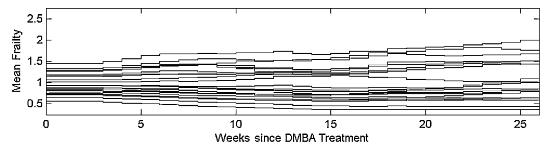
\includegraphics[width=\textwidth]{figure2a.png} % Placeholder
        \caption{}
        \label{fig:2a}
    \end{subfigure}
    \vfill
    \begin{subfigure}[b]{0.8\textwidth}
        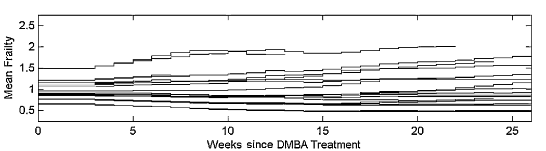
\includegraphics[width=\textwidth]{figure2b.png} % Placeholder
        \caption{}
        \label{fig:2b}
    \end{subfigure}
     \vfill
     \begin{subfigure}[b]{0.8\textwidth}
        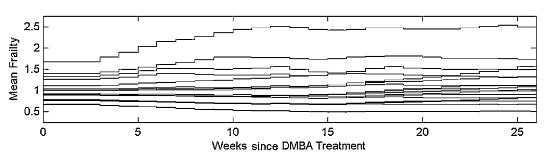
\includegraphics[width=\textwidth]{figure2c.png} % Placeholder
        \caption{}
        \label{fig:2c}
    \end{subfigure}
    \caption{Posterior mean frailty trajectories for animals administered (a) vehicle, (b) 1130 mg/kg canthaxanthin, and (c) 3390 mg/kg canthaxanthin. Figure omits trajectories of animals 67 and 75 in the vehicle group due to their extreme values.}
    \label{fig:2}
\end{figure}


\subsection{Goodness of Fit and Sensitivity Analyses}

Goodness of fit can be assessed by comparing the predictive distribution of the weekly tumor counts with observed values in the data set. As seen in Figure \ref{fig:3}, weekly predictions of tumor incidence prior to sacrifice agree with mortality adjusted means in the data. Assuming sacrifice at week 26, the posterior mean and 95\% credible interval for the number of tumors discovered during the final exam are 0.520 (0.307, 0.808) for the vehicle control group, 0.285 (0.142, 0.509) for the low-dose group, and 0.234 (0.111, 0.420) for the high-dose group, which are in agreement with observed means (0.714, 0.167, and 0.222 tumors for the vehicle, low-dose, and high-dose groups, respectively).

We tested the sensitivity of our methodology to frailty assumptions by comparing the results using the priors from the previous section (denoted DPM1) against the fully parametric dynamic gamma model and the results obtained using an analysis with less confidence in the gamma assumption, expressed by letting $\alpha_{01} = \alpha_{02} = 2$ (DPM2). As seen in Figure \ref{fig:4}, the predictive distributions of the frailties differ somewhat across each model. Most notably, low a priori confidence in the base model causes the distribution of $\phi_{n+1}$ to be more skewed and to have a fatter right tail. However, as seen in Table \ref{tab:sensitivity}, parameter estimates and predictive probabilities are robust.

A second sensitivity analysis was performed for the smoothing parameters by repeating the analysis with $\psi_3 = \psi_4 = 25$ and $\alpha_{01} = \alpha_{02} = 5$ (denoted DPM3). Although Table \ref{tab:sensitivity} demonstrates that lower levels of smoothing decrease the estimated hazard ratios somewhat, conclusions regarding multiplicity and latency effects do not change. In addition, lowering $\psi_3$ and $\psi_4$ does not substantially improve goodness of fit.

\begin{figure}[htbp]
    \centering
     \begin{subfigure}[b]{0.8\textwidth}
        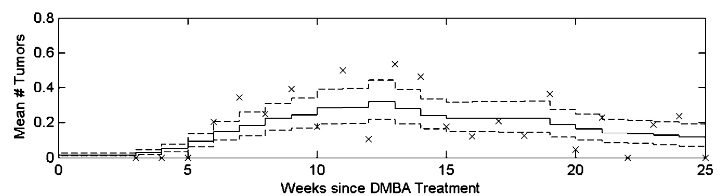
\includegraphics[width=\textwidth]{figure3a.png} % Placeholder
        \caption{}
        \label{fig:3a}
    \end{subfigure}
    \vfill
    \begin{subfigure}[b]{0.8\textwidth}
        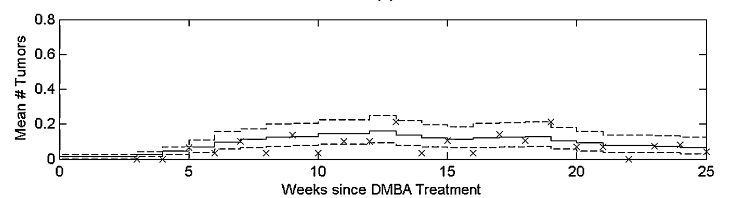
\includegraphics[width=\textwidth]{figure3b.png} % Placeholder
        \caption{}
        \label{fig:3b}
    \end{subfigure}
     \vfill
     \begin{subfigure}[b]{0.8\textwidth}
        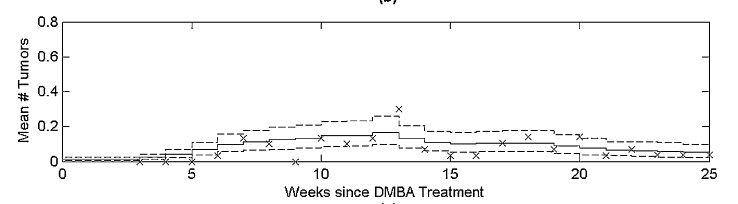
\includegraphics[width=\textwidth]{figure3c.png} % Placeholder
        \caption{}
        \label{fig:3c}
    \end{subfigure}
    \caption{Observed ($\times$) and predicted weekly tumor incidence prior to sacrifice for rats administered (a) vehicle, (b) 1130 mg/kg canthaxanthin, and (c) 3390 mg/kg canthaxanthin. The pointwise 95\% credible intervals (- - -) for the means (---) were calculated based on 1000 draws from the predictive distributions at each iteration of our MCMC algorithm.}
    \label{fig:3}
\end{figure}

\begin{figure}[htbp]
    \centering
     \begin{subfigure}[b]{0.8\textwidth}
        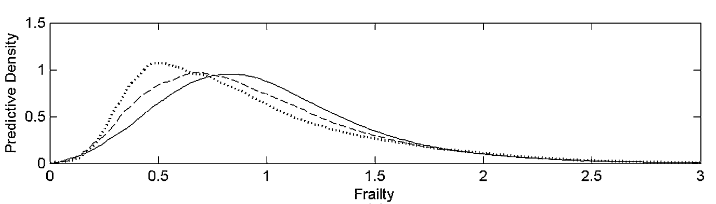
\includegraphics[width=\textwidth]{figure4a.png} % Placeholder
        \caption{}
        \label{fig:4a}
    \end{subfigure}
    \vfill
    \begin{subfigure}[b]{0.8\textwidth}
        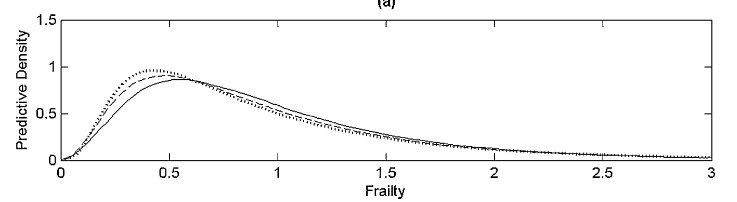
\includegraphics[width=\textwidth]{figure4b.png} % Placeholder
        \caption{}
        \label{fig:4b}
    \end{subfigure}
     \vfill
     \begin{subfigure}[b]{0.8\textwidth}
        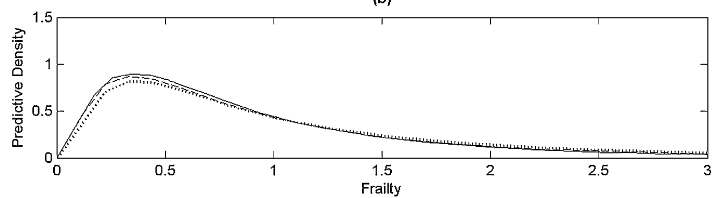
\includegraphics[width=\textwidth]{figure4c.png} % Placeholder
        \caption{}
        \label{fig:4c}
    \end{subfigure}
    \caption{Comparison of predictive frailty distributions obtained using the dynamic gamma model (---), DPM1 (- - -), and DPM2 ($\cdots$). The densities of frailties from intervals (a) 1 ($\phi_{n+1}$), (b) 11 ($\xi_{(n+1)11}$), and (c) 24 ($\xi_{(n+1)24}$) were approximated using a normal kernel smoother (width = 0.05) applied to a posterior sample size of 500,000 (100 draws from the predictive distribution were taken at each iteration).}
    \label{fig:4}
\end{figure}

\begin{table}[htbp]
  \centering
  \caption{Sensitivity analysis of parameter estimates (mean and 95\% credible intervals) and posterior probabilities}
  \label{tab:sensitivity}
  \begin{tabular}{lcccc}
    \toprule
    & \multicolumn{4}{c}{Model} \\
    \cmidrule(lr){2-5}
    Parameter & DPM1 & DPM2 & DPM3 & Dynamic gamma \\
    \midrule
    $\bar{\gamma}_{[10,26]1}$ & 0.489 & 0.485 & 0.420 & 0.482 \\
              & (0.304, 0.758) & (0.304, 0.748) & (0.254, 0.669) & (0.305, 0.735) \\
    $\bar{\gamma}_{[10,26]2}$ & 0.553 & 0.548 & 0.480 & 0.546 \\
              & (0.343, 0.863) & (0.341, 0.855) & (0.289, 0.758) & (0.345, 0.845) \\
    $\omega$    & 7.95 & 7.87 & 7.60 & 8.01 \\
              & (5.34, 11.19) & (5.23, 11.26) & (5.01, 10.82) & (5.41, 11.26) \\
    $\psi_1$    & 5.94 & 5.99 & 5.97 & 5.26 \\
              & (2.03, 12.80) & (2.04, 12.97) & (2.03, 13.02) & (2.03, 12.36) \\
    $\psi_2$    & 48.8 & 48.0 & 49.5 & 50.7 \\
              & (32.4, 69.9) & (31.0, 68.9) & (32.2, 70.5) & (34.0, 70.8) \\
    \midrule
    \multicolumn{1}{l}{Probability} \\
    $P_{M1}$    & 0.999 & $>0.999$ & $>0.999$ & 0.999 \\
    $P_{M2}$    & 0.998 & 0.999 & $>0.999$ & 0.998 \\
    $P_{L1}$    & 0.156 & 0.139 & 0.167 & 0.167 \\
    $P_{L2}$    & 0.392 & 0.360 & 0.399 & 0.394 \\
    \bottomrule
  \end{tabular}
\end{table}


\section{Discussion}

In this article, we have developed a flexible method for inference in multiple event time data. Our method provides a convenient framework for smoothing hazard functions and time-dependent frailty trajectories and covariate effects. An appealing feature of our approach is the incorporation of dynamic frailties with nonparametric distributions. Even in a data set comprised of fairly homogeneous animals, our model is capable of identifying age-dependent shifts in susceptibility. By comparing the individuals' frailty trajectories, one can identify unusual individuals for genotyping and further examination. However, even in applications where the frailty is of no interest to the researcher, it would still be necessary to account for these trends to improve the accuracy of future predictions.

Although our proposed method accommodates a wide variety of time-dependent trends and distributions, the computational burden may not pay off in certain situations. In particular, studies of rare events or with few exam times may have minimal information in the data about time-varying frailty distributions. Although one could still apply our method in such a case, there may be minimal Bayesian learning and the prior would be utilized strongly in extrapolating over time. In these situations, a simple frequentist analysis may suffice.

By using DP priors for a shared frailty and multiplicative innovations on the frailty, we have provided a less restrictive modeling framework than parametric alternatives. As mentioned previously, these priors ensure that the posterior distributions of the frailties are almost surely discrete \citep{Blackwell1973}. This restriction could be removed by using P\'olya tree priors \citep{Lavine1992, Lavine1994} instead of the DP, as was done by \citet{Walker1997} in the context of a shared frailty. However, a simpler alternative would be to model each $\phi_i$ and $\phi_{ij}$ using a DP mixture. Although we did not consider such a methodology, this would be straightforward because it would just involve adding another level to the hierarchy.

Several extensions of our method would be interesting to pursue. For example, one could consider priors with a mixture structure to allow selection of the frailty form, in particular, selection between no frailty, a shared frailty, and a dynamic frailty for each predictor. This approach would be a generalization of recent work by \citet{Dunson2004}. A formal method for testing for lack of fit of the dynamic gamma model would also be of interest. For instance, \citet{Berger2001}'s method for comparing parametric and nonparametric models could potentially be adapted to our framework. The results from these lack-of-fit tests could be used to determine whether the dynamic gamma model, or our nonparametric extension, should be used for data from similar studies. Another possible direction would be to apply our nonparametric framework to allow dynamic random effects in generalized linear models for longitudinal data and for joint modeling of longitudinal and survival data.

% --- Acknowledgements ---
\section*{Acknowledgements}
The authors thank Dr Clinton Grubbs, University of Alabama at Birmingham, for providing the data and Bo Cai and Gregg Dinse for their helpful comments. This research was supported by the Intramural Research Program of the NIH, and NIEHS.

% --- Bibliography ---
\bibliographystyle{plainnat} % Choose a suitable natbib style
\bibliography{references} % Your .bib file name

\newpage % Ensure Received/Revised/Accepted is on a new page if needed
\noindent Received August 2005. Revised November 2005. Accepted January 2006.

\end{document}
% --- Document End ---